%*************************************************************************
\section{Voraussetzung und Installation}
%*************************************************************************

SiLift ist als \textit{Eclipse-Feature} unter folgender \textit{Update-Site} erhältlich:\\ \url{http://pi.informatik.uni-siegen.de/Projekte/SiLift/updatesite}.\\


\textbf{Hinweis:} Vergewissern Sie sich, ob ihr Eclipse die notwendigen Voraussetzungen erfüllt. 
Eine Liste der benötigten Plugins ist unter \url{http://pi.informatik.uni-siegen.de/Projekte/SiLift/download.php} zu finden.
Bitte beachten Sie dabei die entsprechenden Hinweise zu den jeweiligen Versionen.\\


Sofern alle Voraussetzungen erfüllt sind, kann SiLift wie gewohnt über den Menüpunkt \texttt{Help} $\triangleright$ \texttt{Install New Software...} installiert werden (vgl. Abb. \ref{eclipse-install_new_software}).

\begin{figure}[H]
\centering
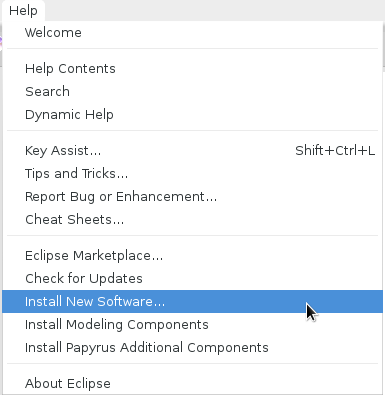
\includegraphics[width=0.25\textwidth]{requirements/graphics/eclipse-install_new_software.png}
\caption{Eclipse: Install New Software...}
\label{eclipse-install_new_software}
\end{figure}

Es sollten Ihnen vier Kategorien angezeigt werden (vgl. Abb. \ref{eclipse-install_silift}). 

\begin{figure}[H]
\centering
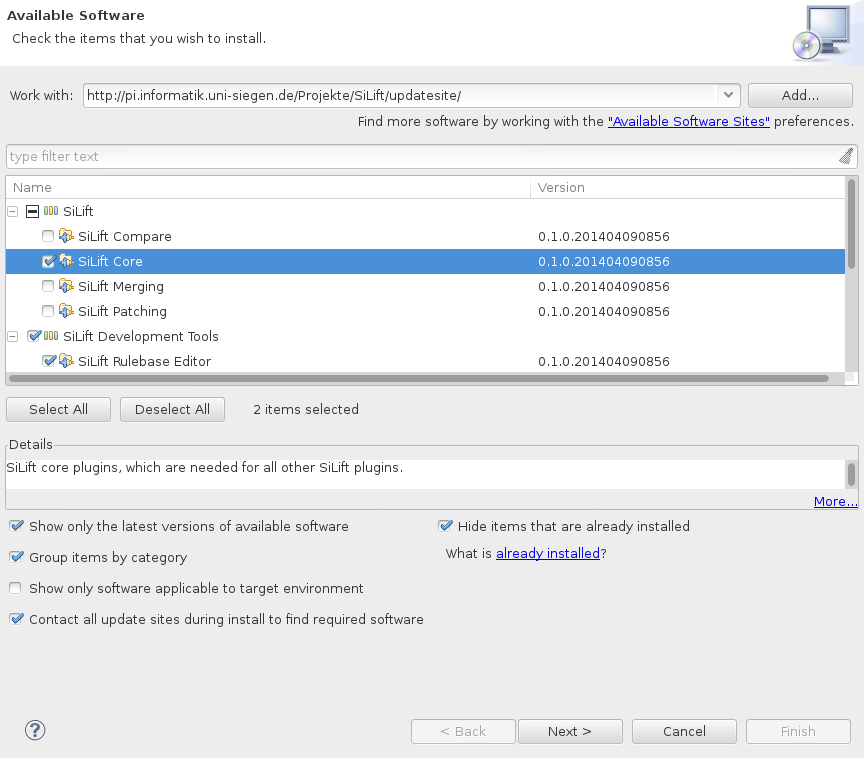
\includegraphics[width=0.6\textwidth]{requirements/graphics/eclipse-install_silift.png}
\caption{SiLift Update Site}
\label{eclipse-install_silift}
\end{figure}

Für die folgenden Tutorials benötigen das Feature \texttt{SiLift Core} aus der Kategorie \texttt{SiLift} und das Feature \texttt{SiLift Rule Base Editor} aus der Kategorie \texttt{SiLift Development Tools}. Danach klicken Sie auf \texttt{Next} und folgen dem Installationsassistenten.
